\documentclass[11pt, a4paper, journal]{paper}

\usepackage[bottom = 2.5cm, top = 2.5cm, inner= 2cm, outer = 1.5cm]{geometry}

\usepackage[utf8]{inputenc} 	 
\usepackage[T5]{fontenc} 
\usepackage[vietnamese]{babel}
 
\usepackage{amssymb, amsthm}
\usepackage[intlimits]{mathtools}
\usepackage{graphicx}

\usepackage{float}
\usepackage{multicol}

\def\submit{\small (Nhận ngày:..., Đăng ngày:...)}

%%%%%%%%%%%%%%%%
\begin{document}

\title{Xác định tỷ số ISOMER bằng thực nghiệm}

\author{Trần Trí Viễn\textsuperscript{a,b}\thanks{email: abc@gmail.com \newline tel: 0912345678}~, 
	Đoàn Quang Tuyền\textsuperscript{b}, 
	Nguyễn Trung Tính\textsuperscript{b}, 
	Nguyễn Văn A\textsuperscript{a}
}
\institution{
	\textsuperscript{a}Viện nghiên cứu hạt nhân,\\
	\textsuperscript{b}Đại học khoa học tự nhiên
}

\date{\submit}

\shortauthor{Trần Trí Viễn, Đoàn Quang Tuyền, Nguyễn Trung Tính, Nguyễn Văn A}
\shorttitle{Xác định tỷ số ISOMER bằng thực nghiệm}
\oddrunhead{T. T. Vien et al.}
\evenrunhead{Xác định tỷ số ISOMER bằng thực nghiệm}

\maketitle

\begin{abstract}
Tóm tắt nội dung của bài báo, nêu vấn đề, cách giải quyết vấn đề, các kết quả chính và kết luận, kiến nghị, v.v. Tóm tắt nội dung của bài báo, nêu vấn đề, cách giải quyết vấn đề, các kết quả chính và kết luận, kiến nghị ... 
\end{abstract}

\begin{keywords}
Tỷ số ISOMER, phổ gamma, ghi nhận bức xạ.
\end{keywords}

%%%%%%%%%%
\begin{multicols}{2}

\section{Mở đầu}
Các hạt nhân $^{44}Sc$ được tạo thành thông qua phản ứng:

\begin{equation}
\gamma + ^{46}Ti \rightarrow ^{44}Sc + n + p
\end{equation}

Trình bày các đoạn văn bản và các công thức toán học hoặc hình vẽ có liên quan tới nội dung của để mục giống như đôi với luận văn, luận án, hoặc các bài báo cáo. Trình bày các đoạn văn bản và các công thức toán học hoặc hình vẽ có liên quan tới nội dung của để mục giống như đôi với luận văn, luận án, hoặc các bài báo cáo. Trình bày các đoạn văn bản và các công thức toán học hoặc hình vẽ có liên quan tới nội dung của để mục giống như đôi với luận văn, luận án, hoặc các bài báo cáo ... 

\section{Tính toán các thông số của phản ứng}
Các thông số của phản ứng được trình bày trong tài liệu \cite{bib_boston1997, bib_Klein, bib_Knoll} ....

Trình bày các đoạn văn bản và các công thức toán học hoặc hình vẽ có liên quan tới nội dung của để mục giống như đôi với luận văn, luận án, hoặc các bài báo cáo. Trình bày các đoạn văn bản và các công thức toán học hoặc hình vẽ có liên quan tới nội dung của để mục giống như đôi với luận văn, luận án, hoặc các bài báo cáo. Trình bày các đoạn văn bản và các công thức toán học hoặc hình vẽ có liên quan tới nội dung của để mục giống như đôi với luận văn, luận án, hoặc các bài báo cáo ... 

\section{Thí nghiệm}
Mô hình thí nghiệm được thể hiện trên Hình \ref{fig:exp} ...

\begin{figure}[H]
\centering
	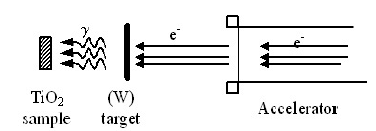
\includegraphics[width=0.7\linewidth]{exp.png}
	\caption{Bố trí thí nghiệm.}
	\label{fig:exp}
\end{figure}

Trình bày các đoạn văn bản và các công thức toán học hoặc hình vẽ có liên quan tới nội dung của để mục giống như đôi với luận văn, luận án, hoặc các bài báo cáo. Trình bày các đoạn văn bản và các công thức toán học hoặc hình vẽ có liên quan tới nội dung của để mục giống như đôi với luận văn, luận án, hoặc các bài báo cáo. Trình bày các đoạn văn bản và các công thức toán học hoặc hình vẽ có liên quan tới nội dung của để mục giống như đôi với luận văn, luận án, hoặc các bài báo cáo ... 

\section{Kết quả thực nghiệm}
Kết quả thực nghiệm được trình bày ...

 Trình bày các đoạn văn bản và các công thức toán học hoặc hình vẽ có liên quan tới nội dung của để mục giống như đôi với luận văn, luận án, hoặc các bài báo cáo. Trình bày các đoạn văn bản và các công thức toán học hoặc hình vẽ có liên quan tới nội dung của để mục giống như đôi với luận văn, luận án, hoặc các bài báo cáo. Trình bày các đoạn văn bản và các công thức toán học hoặc hình vẽ có liên quan tới nội dung của để mục giống như đôi với luận văn, luận án, hoặc các bài báo cáo ... 

\section{Kết luận}
Trình bày kết luận...

Trình bày các đoạn văn bản và các công thức toán học hoặc hình vẽ có liên quan tới nội dung của để mục giống như đôi với luận văn, luận án, hoặc các bài báo cáo. Trình bày các đoạn văn bản và các công thức toán học hoặc hình vẽ có liên quan tới nội dung của để mục giống như đôi với luận văn, luận án, hoặc các bài báo cáo. Trình bày các đoạn văn bản và các công thức toán học hoặc hình vẽ có liên quan tới nội dung của để mục giống như đôi với luận văn, luận án, hoặc các bài báo cáo ... 

\section{Lời cảm ơn}
Phần Lời cảm ơn ...

Trình bày các đoạn văn bản và các công thức toán học hoặc hình vẽ có liên quan tới nội dung của để mục giống như đôi với luận văn, luận án, hoặc các bài báo cáo. Trình bày các đoạn văn bản và các công thức toán học hoặc hình vẽ có liên quan tới nội dung của để mục giống như đôi với luận văn, luận án, hoặc các bài báo cáo. Trình bày các đoạn văn bản và các công thức toán học hoặc hình vẽ có liên quan tới nội dung của để mục giống như đôi với luận văn, luận án, hoặc các bài báo cáo ... 

\bibliographystyle{ieeetr}
\bibliography{ttvien_biblio}

\end{multicols}

\end{document}